\documentclass[twoside]{article}

\usepackage[preprint]{aistats2027}
\usepackage[round,authoryear]{natbib}
\usepackage{amsmath,amssymb,amsthm}
\usepackage{mathtools}
\usepackage{microtype}
\usepackage{booktabs}
\usepackage{graphicx}
\usepackage{url}

\renewcommand{\bibname}{References}
\renewcommand{\bibsection}{\subsubsection*{\bibname}}
\bibliographystyle{apalike}

\newtheorem{theorem}{Theorem}
\newtheorem{proposition}[theorem]{Proposition}
\newtheorem{corollary}[theorem]{Corollary}
\newtheorem{lemma}[theorem]{Lemma}
\newtheorem{remark}[theorem]{Remark}
\newcommand{\E}{\mathbb E}
\newcommand{\R}{\mathbb R}
\newcommand{\Var}{\operatorname{Var}}
\newcommand{\tr}{\operatorname{tr}}
\newcommand{\rank}{\operatorname{rank}}
\newcommand{\op}{\mathrm{op}}
\newcommand{\cL}{\mathcal L}
\newcommand{\OPT}{\mathrm{OPT}}

\begin{document}
\runningauthor{}

\twocolumn[
\aistatstitle{Pure Relative Structured Matrix Learning with Square-Root Matvecs}

\aistatsauthor{Pahan Dewasurendra}

\aistatsaddress{Johns Hopkins University}
]

\begin{abstract}
Let $\cL\subseteq\R^{n\times m}$ be any known $q$-dimensional linear matrix
family, and let an unknown $A$ be accessible only through products $Ax$ and
$A^\top y$. A recent result obtains a nearly optimal approximation from
$\cL$ in about $\sqrt q$ queries, but incurs factor three and additive error
proportional to $\|A\|_F$. Whether sublinear query complexity can give pure
$(1+\epsilon)$ relative error was left open.

We resolve this problem with a polynomial-time, nonadaptive algorithm. For a
Frobenius-orthonormal basis $B_1,\ldots,B_q$, form the basis-invariant partial
trace $S_L=\sum_iB_iB_i^\top$. The algorithm queries the leading eigenspace
of $S_L$ exactly from the left, then fits the remaining directions from a
Gaussian right sketch. If $\lambda_j$ are the eigenvalues of $S_L$, its
constant-success query complexity is
\[
 \min_s\left\{s+C\left[
 \begin{aligned}
 &\max\{1,\lambda_{s+1}\}\log^2(2q)\\
 &+\lambda_{s+1}/\epsilon
 \end{aligned}\right]\right\}.
\]
The transposed profile is also available. Since
$\lambda_{s+1}\le q/(s+1)$, every family admits pure relative error with
$\widetilde O(\sqrt{q/\epsilon})$ queries, independent of ambient dimensions
and $\|A\|_F/\OPT$. The key proof is a partial-trace covariance lemma for a
Gaussian matrix-valued design. Exact high-leverage queries make its expected
Hessian the identity, while the centered regression offset has variance only
$O(\lambda_{s+1}\OPT^2/k)$. A median construction amplifies success without
estimating residual norms. Finally, a symmetric Wishart lower bound for
fixed-sparsity approximation yields $\Omega(\sqrt{q/\epsilon})$ adaptive
two-sided queries when $q\epsilon$ is bounded below. Thus the universal rate
is optimal up to logarithmic factors in this joint regime. We also show that
the transformed profile gives pure relative reducible prediction risk under known
input and output covariances. For structured positive-definite precisions, it
further controls Gaussian KL error and preconditioned condition number.
\end{abstract}

\section{Introduction}

Matrix-vector products are the basic access primitive for implicit Hessians,
linear predictors, kernel matrices, and matrix functions. When a
matrix $A$ is too large to form, one may still apply $x\mapsto Ax$ and, when
an adjoint is available, $y\mapsto A^\top y$. This motivates a statistical
question: how many such queries reveal the best structured approximation to
$A$?

This question includes a structured prediction problem. If
$Y=AX+\eta$ and only input-output experiments with the unknown linear operator
are available, then approximating $A$ under the covariance of $X$ is exactly
approximating the reducible prediction risk. It also includes matrix-free
curvature compression: automatic differentiation supplies Hessian-vector
products without materializing a Hessian, while a structured precision can
define a scalable Gaussian approximation or preconditioner. Our results apply
agnostically in both cases. The target operator need only be near the proposed
structure.

We study a known linear matrix family $\cL\subseteq\R^{n\times m}$ of
dimension $q$. Given two-sided matvec access to an arbitrary $A$, the goal is
to return $\widehat B\in\cL$ such that
\begin{equation}
 \|A-\widehat B\|_F
 \le (1+\epsilon)\min_{B\in\cL}\|A-B\|_F.
 \label{eq:goal}
\end{equation}
The target is agnostic. No stochastic noise model or promise that
$A\in\cL$ is imposed.

\citet{amsel2026query} initiated a general theory for this problem. For a
finite family $\mathcal F$, they give a nearly quadratic improvement from
$O(\log|\mathcal F|)$ one-sided queries to
$\widetilde O(\sqrt{\log|\mathcal F|})$ two-sided queries. Covering a linear
family gives roughly $\sqrt q$ queries, but the guarantee is
\begin{equation}
 (3+\epsilon)\OPT+\alpha\|A\|_F.
 \label{eq:prior}
\end{equation}
They explicitly ask whether every $q$-dimensional linear family admits pure
$(1+\epsilon)$ error with
$\widetilde O(\sqrt q/\operatorname{poly}(\epsilon))$ queries, and whether
this can be achieved in polynomial time.

The obstruction is not identifiability. In the realizable case, generic
queries often recover a linear family exactly
\citep{halikias2024structured}. The difficulty is an arbitrary
orthogonal residual. A direct Gaussian least-squares fit has an unbiased
normal equation, but a few matrix contractions need not embed all $q$
parameter directions. Requiring a conventional subspace embedding returns
to order $q$ queries.

Our solution separates the directions that actually obstruct concentration.
Let $B_1,\ldots,B_q$ be a Frobenius-orthonormal basis of $\cL$ and define
\begin{equation}
 S_L=\sum_{i=1}^q B_iB_i^\top,
 \qquad
 S_R=\sum_{i=1}^q B_i^\top B_i.
 \label{eq:partial-traces}
\end{equation}
These partial traces are basis invariant, positive semidefinite, and have
trace $q$. We query a leading eigenspace of one partial trace exactly. On its
orthogonal complement, Gaussian matvecs have both a well-conditioned Hessian
and a small regression offset. The first fact costs the remaining spectral
leverage times logarithmic factors. The second costs the same leverage divided
by $\epsilon$. Optimizing where to split gives square-root complexity.

\paragraph{Contributions.}
Our principal results are theoretical.
\begin{itemize}
\item We give a nonadaptive, polynomial-time algorithm satisfying
\eqref{eq:goal} for every rectangular linear family. Its query complexity is
the better of two basis-invariant spectral profiles, one for each query
orientation.

\item The profile implies a universal
$\widetilde O(\sqrt{q/\epsilon})$ upper bound. It has no additive error and no
dependence on the ambient dimensions or the ratio $\|A\|_F/\OPT$.

\item We prove a Gaussian covariance lemma controlled by a partial trace. The
proof combines a dimension-free Schatten moment estimate, an exact
fourth-moment calculation, and matrix concentration for unbounded summands.

\item We convert the adaptive symmetric Wishart lower bound of
\citet{amsel2026fixed} into
$\Omega(\sqrt{q/\epsilon})$ for general $q$-dimensional linear families when
$q\epsilon=\Omega(1)$. This matches our upper bound up to logarithms. A
separate GOE construction shows that $\Omega(1/\sqrt\epsilon)$ queries can be
necessary even for a one-dimensional family.

\item We lift the theorem to covariance-weighted prediction loss without
changing its query count. For positive-definite precision matrices, the same
output controls both Gaussian KL divergence and preconditioning quality.
Circulant, Toeplitz, and known-graph precision families give explicit
dimension-adaptive profiles.
\end{itemize}

\paragraph{Why two sides matter.}
The partial trace identifies output directions shared by many basis matrices.
A left query reveals one such direction exactly, no matter how many
coefficients use it. Gaussian right queries then handle the diffuse
remainder. Strong one-sided barriers are known for general matrix-free tasks
\citep{halikias2026transpose}. Our estimator makes the complementary roles of
the two orientations explicit.

Table~\ref{tab:comparison} separates the guarantee and query dependence of the
closest general result. The earlier linear-family
bound is obtained by covering a bounded part of $\cL$, then running a
finite-candidate procedure. Its runtime scales with the cover size. Our
algorithm instead solves linear least squares in the original $q$
coefficients.

\begin{table}[t]
\centering
\caption{General $q$-dimensional linear families. Logarithmic factors other
than $\log(1/\alpha)$ are suppressed.}
\label{tab:comparison}
\small
\begin{tabular}{lcc}
\toprule
Result & Queries & Guarantee \\
\midrule
Amsel et al. &
$\frac{\sqrt{q\log(1/\alpha)}}{\epsilon^2}$ &
$(3+\epsilon)\OPT+\alpha\|A\|_F$ \\
This paper & $\sqrt{q/\epsilon}$ & $(1+\epsilon)\OPT$ \\
\bottomrule
\end{tabular}
\end{table}

\section{Why a Spectral Split Is Necessary}
\label{sec:obstruction}

It is tempting to fit $\cL$ using only a right Gaussian sketch, or only a
left sketch, then choose whichever orientation has smaller aggregate
variance. This cannot prove a square-root theorem. For an orthonormal basis,
define the two offset leverages of a residual $R\perp\cL$ by
\begin{equation}
 V_R(R)=\sum_i\|R^\top B_i\|_F^2,
 \qquad
 V_L(R)=\sum_i\|RB_i^\top\|_F^2.
 \label{eq:offset-leverages}
\end{equation}
A one-sided Gaussian normal equation has total offset variance proportional
to the corresponding quantity. One might hope that
$\min\{V_R,V_L\}=O(\sqrt q\|R\|_F^2)$, or that their product is at most
$q\|R\|_F^4$. Both statements are false.

\begin{proposition}[Deleted-tangent obstruction]
\label{prop:tangent}
For every $a,b\ge1$, there is a linear family of dimension $q=a+b$ and a
unit residual $R\perp\cL$ such that
\[
 V_R(R)=b,
 \qquad V_L(R)=a.
\]
When $a$ and $b$ are comparable, both global orientations have order-$q$
offset variance. Nevertheless, the spectral-split estimator removes all
contamination with one exact query.
\end{proposition}

\begin{proof}
Let $u,e_1,\ldots,e_a$ and $v,f_1,\ldots,f_b$ be orthonormal systems. Take
$R=uv^\top$ and let $\cL$ have orthonormal basis
\begin{equation}
 \{uf_j^\top:1\le j\le b\}
 \mathbin\cup
 \{e_iv^\top:1\le i\le a\}.
 \label{eq:tangent-family}
\end{equation}
The deleted matrix $uv^\top$ is orthogonal to every basis element. For the
first arm, $\|R^\top(uf_j^\top)\|_F=1$, while the corresponding terms from
the second arm vanish. This gives $V_R=b$. The transposed calculation gives
$V_L=a$.

The left partial trace is
\[
 S_L=buu^\top+\sum_{i=1}^ae_ie_i^\top.
\]
Querying $u$ exactly leaves partial-trace norm one. More strongly, the
remaining residual is $(I-uu^\top)R=0$, so the random-stage offset vanishes.
\end{proof}

This example isolates the role of the deterministic term in
\eqref{eq:estimator}. It is not included to obtain a conventional subspace
embedding. It makes the high-curvature and high-offset directions exact,
which leaves a centered problem whose variance is governed by the residual
partial trace. A fixed global choice of orientation misses this local
structure.

\section{Problem and Algorithm}
\label{sec:algorithm}

Let $\cL\subseteq\R^{n\times m}$ have Frobenius-orthonormal basis
$B_1,\ldots,B_q$. Write
\[
 B_\star=P_{\cL}A,
 \qquad R=A-B_\star,
 \qquad \OPT=\|R\|_F.
\]
Then $\langle R,B\rangle_F=0$ for every $B\in\cL$. For the left partial trace
$S_L$, let
$\lambda_1^L\ge\lambda_2^L\ge\cdots\ge0$ be its eigenvalues, padded by
zeros. Fix $s\in\{0,\ldots,n\}$, let $P$ project onto its first $s$
eigenvectors, set $Q=I-P$, and abbreviate
$\lambda=\lambda_{s+1}^L=\|QS_LQ\|_\op$.

If $\lambda=0$, query $A^\top$ on an orthonormal basis of
$\operatorname{range}(P)$ and
minimize $\|P(A-B)\|_F^2$ over $B\in\cL$. This recovers $B_\star$ because
$QB=0$ for every $B\in\cL$.

Suppose $\lambda>0$. In addition to the same $s$ left queries, draw
$G=[g_1,\ldots,g_k]\in\R^{m\times k}$ with independent standard Gaussian
entries and issue the $k$ right queries $Ag_\ell$. Return the minimum-norm
minimizer
\begin{equation}
 \widehat B\in\arg\min_{B\in\cL}
 \left\{
 \|P(A-B)\|_F^2+\frac1k\|Q(A-B)G\|_F^2
 \right\}.
 \label{eq:estimator}
\end{equation}
The objective is observable. The left responses give $PA$, and $QAG$ is
obtained from $AG-PAG$. Equation \eqref{eq:estimator} is an ordinary
$q$-variable least-squares problem.

Define the one-orientation profile
\begin{equation}
 \begin{aligned}
 \mathsf Q_L(\epsilon)=\min_{0\le s\le n}\biggl\{s+C\biggl[
 &\max\{1,\lambda_{s+1}^L\}\log^2(2q)\\
 &+\frac{\lambda_{s+1}^L}{\epsilon}
 \biggr]\biggr\},
 \end{aligned}
 \label{eq:left-profile}
\end{equation}
where the bracketed term is zero if $\lambda_{s+1}^L=0$. Define
$\mathsf Q_R(\epsilon)$ analogously from $S_R$. The right profile swaps the
roles of $A$ and $A^\top$.

\begin{theorem}[Pure relative profile]
\label{thm:profile}
For every $A\in\R^{n\times m}$, every $q$-dimensional linear family $\cL$,
and every $\epsilon\in(0,1)$, the better orientation of
\eqref{eq:estimator} returns $\widehat B\in\cL$ satisfying
\eqref{eq:goal} with probability at least $0.9$ using at most
\[
 \min\{\mathsf Q_L(\epsilon),\mathsf Q_R(\epsilon)\}
\]
matvec queries. The query vectors are nonadaptive and the estimator runs in
time polynomial in the explicit input size of the basis.

For failure probability $\delta$, multiply only the bracketed random-query
term in \eqref{eq:left-profile} by $C\log(1/\delta)$, and likewise for the
right profile.
\end{theorem}

\paragraph{Computation model.}
The polynomial-time statement uses real arithmetic and an explicit linearly
independent basis. A nonorthonormal basis is whitened through its $q\times q$
Frobenius Gram matrix. The partial trace is then formed explicitly, a symmetric
eigenproblem is solved, and \eqref{eq:estimator} is a least-squares problem in
$q$ unknowns. No eigengap is required: for any computed rank-$s$ projector,
the guarantee holds with the directly certifiable residual leverage
$\Lambda_L(P)$ in \eqref{eq:projector-profile}. On the covariance event the
least-squares Hessian has smallest eigenvalue at least $1/2$. Bit complexity
still depends on the conditioning of the supplied basis, which we do not hide
inside the query bound.

The leading eigenspace is not merely convenient. It is the best rank-$s$
choice for this estimator. For an arbitrary rank-$s$ orthogonal projector
$P$, define its residual leverage
\begin{equation}
 \Lambda_L(P)=\|(I-P)S_L(I-P)\|_\op.
 \label{eq:projector-leverage}
\end{equation}
The same proof as Theorem~\ref{thm:profile} gives query count
\begin{equation}
 s+C\left[
 \max\{1,\Lambda_L(P)\}\log^2(2q)
 +\frac{\Lambda_L(P)}{\epsilon}
 \right].
 \label{eq:projector-profile}
\end{equation}

\begin{proposition}[Optimal exact-query subspace]
\label{prop:optimal-projector}
Among all rank-$s$ orthogonal projectors $P$,
\[
 \min_{\rank(P)=s}\Lambda_L(P)=\lambda_{s+1}^L.
\]
Thus the leading eigenspace minimizes both random-query terms in
\eqref{eq:projector-profile}.
\end{proposition}

\begin{proof}
For $Q=I-P$, $\Lambda_L(P)$ is the largest Rayleigh quotient of $S_L$ on
$\operatorname{range}(Q)$. The claim is the Courant--Fischer characterization of
$\lambda_{s+1}^L$.
\end{proof}

\begin{corollary}[Universal square-root bound]
\label{cor:universal}
Let $L_\epsilon=\log^2(2q)+1/\epsilon$. Constant-success pure relative error
requires at most
\begin{equation}
 O\!\left(\sqrt{qL_\epsilon}+\log^2(2q)\right)
 =\widetilde O\!\left(\sqrt{q/\epsilon}\right)
 \label{eq:universal}
\end{equation}
two-sided matvec queries.
\end{corollary}

\begin{proof}
The partial-trace eigenvalues sum to $q$, so
$\lambda_{s+1}^L\le q/(s+1)$. Also
$\max\{1,\lambda\}\le1+\lambda$. Insert these inequalities into
\eqref{eq:left-profile} and choose
$s=\min\{n,\lfloor\sqrt{qL_\epsilon}\rfloor\}$. If this choice reaches $n$,
the exact queries already cover the row support of $\cL$. Otherwise the two
$s$-dependent terms are both $O(\sqrt{qL_\epsilon})$.
\end{proof}

\section{Statistical Consequences and Concrete Profiles}
\label{sec:statistics}

The Frobenius objective is not tied to isotropic inputs. Let
$\Gamma\succ0$ and $\Omega\succ0$ be known input and output weights and define
\begin{equation}
 \|M\|_{\Omega,\Gamma}^2
 =\|\Omega^{1/2}M\Gamma^{1/2}\|_F^2.
 \label{eq:weighted-norm}
\end{equation}
Transform the operator and family by
$A'=\Omega^{1/2}A\Gamma^{1/2}$ and
$\cL'=\Omega^{1/2}\cL\Gamma^{1/2}$. A right query to $A'$ is implemented by
querying $A$ at $\Gamma^{1/2}g$, then multiplying the response by
$\Omega^{1/2}$. A left query is implemented analogously. Thus whitening costs
no additional oracle calls.

\begin{corollary}[Structured prediction risk]
\label{cor:prediction}
Let $Y=AX+\eta$, where $\E[\eta\mid X]=0$ and
$\E[XX^\top]=\Gamma$. Given two-sided queries to $A$, the transformed profile
of Theorem~\ref{thm:profile} returns $\widehat B\in\cL$ such that
\begin{multline}
 \E\|\Omega^{1/2}(Y-\widehat BX)\|_2^2-\mathsf N\\
 \le(1+\epsilon)\min_{B\in\cL}
 \left\{\E\|\Omega^{1/2}(Y-BX)\|_2^2-\mathsf N\right\},
 \label{eq:prediction-risk}
\end{multline}
with probability at least $0.9$, where
$\mathsf N=\E\|\Omega^{1/2}\eta\|_2^2$. The profile uses a basis orthonormal
under \eqref{eq:weighted-norm} and its corresponding weighted partial traces.
\end{corollary}

\begin{proof}
The conditional mean assumption gives
$\E\|\Omega^{1/2}(Y-BX)\|_2^2
=\mathsf N+\|A-B\|_{\Omega,\Gamma}^2$.
Apply Theorem~\ref{thm:profile} to $(A',\cL')$ with
$\epsilon'=\sqrt{1+\epsilon}-1\ge\epsilon/3$, then square its guarantee.
Replacing $\epsilon$ by $\epsilon'$ changes the profile by only a universal
constant.
\end{proof}

This statement is distribution-free beyond second moments. Gaussian probes
are an experimental design chosen by the algorithm, not an assumption on
$X$. The result is therefore an oracle-complexity theorem for the best
structured linear predictor under a specified deployment covariance.

For Gaussian uncertainty quantification, the matrix approximation also has a
direct distributional consequence.

\begin{corollary}[Structured Gaussian precision]
\label{cor:precision}
Suppose $A=A^\top\succeq\mu I$, every matrix in $\cL$ is symmetric, and set
$r=(1+\epsilon)\OPT/\mu<1$. The output of
Theorem~\ref{thm:profile} is positive definite and satisfies
\begin{align}
 \mathrm{KL}\!\left(N(0,A^{-1})\,\|\,N(0,\widehat B^{-1})\right)
 &\le \frac{(1+\epsilon)^2\OPT^2}{4\mu^2(1-r)},
 \label{eq:kl-bound}\\
 \kappa(\widehat B^{-1/2}A\widehat B^{-1/2})
 &\le\frac{1+r}{1-r}.
 \label{eq:precondition-bound}
\end{align}
\end{corollary}

\begin{proof}
Let $E=A^{-1/2}(\widehat B-A)A^{-1/2}$. Then
$\|E\|_\op\le r$, which proves positive definiteness and
\eqref{eq:precondition-bound}. If $e_i$ are the eigenvalues of $E$, the KL
divergence is $\frac12\sum_i[e_i-\log(1+e_i)]$. For
$|e_i|\le r$, the summand is at most $e_i^2/[2(1-r)]$. Finally,
$\|E\|_F\le\|A-\widehat B\|_F/\mu$.
\end{proof}

Table~\ref{tab:profiles} makes the spectral profile explicit for statistical
structures. For real Toeplitz matrices, the normalized diagonal basis gives
the $i$th partial-trace entry
$H_n-H_{i-1}+H_{n-1}-H_{n-i}$, so its maximum is $H_n$. For a known graph
precision model, use $E_{ii}$ on vertices and
$(E_{ij}+E_{ji})/\sqrt2$ on edges. The partial trace is diagonal with entry
$1+\deg(i)/2$. Exact queries can therefore remove hubs before the random
stage.

\begin{table}[t]
\centering
\caption{Constant-success profile examples. Tildes hide logarithmic factors.}
\label{tab:profiles}
\small
\begin{tabular}{lccc}
\toprule
Family & $q$ & $\|S_L\|_\op$ & Queries \\
\midrule
Circulant & $n$ & $1$ & $\widetilde O(1/\epsilon)$ \\
Toeplitz & $2n-1$ & $H_n$ & $\widetilde O(\log n/\epsilon)$ \\
Graph precision & $n+|E|$ & $1+\Delta/2$ & $\widetilde O((1+\Delta)/\epsilon)$ \\
$a\times b$ block & $ab$ & $b$ & $\min\{a,b\}$ exact \\
\bottomrule
\end{tabular}
\end{table}

For diagonal matrices, $S_L=I$ and the random stage similarly uses
$O(\log^2q+1/\epsilon)$ queries, matching specialized dimension-free behavior
up to logarithms \citep{amsel2026fixed,dharangutte2023tight}. For an arbitrary
coordinate subspace, the partial traces are row and column degree matrices.
Graph degeneracy can give a sharper sparse-only profile
\citep{musco2026instance}, while our theorem also covers dense overlapping
bases and weighted prediction loss.

Figure~\ref{fig:profiles} is a small falsification check rather than evidence
for the theorem. We generated a unit random residual, projected it exactly
orthogonal to each family, and solved the right-sketch least-squares problem
over 120 independent sketches. The median squared excess follows the predicted
$1/k$ behavior once the random design is nonsingular. Dotted curves show the
90th percentile. The supplement gives the complete protocol and seed.

\begin{figure}[t]
 \centering
 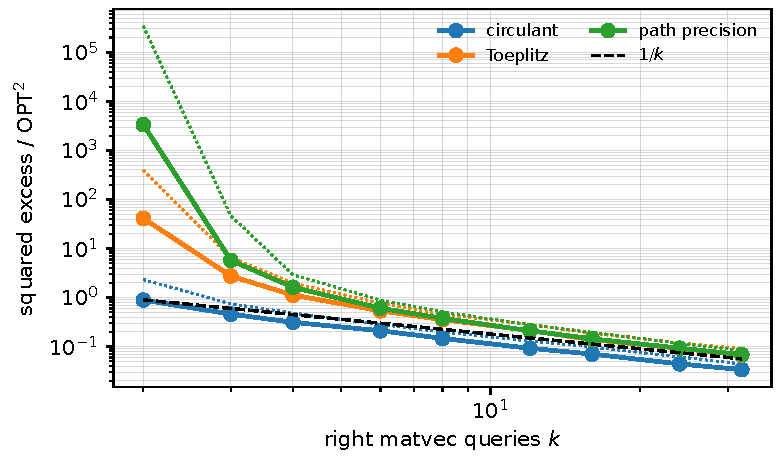
\includegraphics[width=\columnwidth]{profile_experiment.pdf}
 \caption{Relative squared excess for three $32\times32$ families. The dashed
 line has slope $1/k$.}
 \label{fig:profiles}
\end{figure}

\section{Proof of the Upper Bound}
\label{sec:proof}

We give the main argument and defer moment details and amplification to the
supplement. Set $C_i=QB_i$ and define the $q\times q$ Gram matrix
\[
 K_{ij}=\langle C_i,C_j\rangle_F.
\]
Since the original basis is orthonormal, $0\preceq K\preceq I$. Moreover,
\begin{equation}
 \sum_{i=1}^q C_iC_i^\top=QS_LQ\preceq\lambda I.
 \label{eq:leverage-control}
\end{equation}
For $g\sim N(0,I_m)$, let $D(g)\in\R^{n\times q}$ have columns $C_ig$.

\begin{lemma}[Partial-trace Gaussian covariance]
\label{lem:covariance}
Suppose $K\preceq I$ and
$\sum_iC_iC_i^\top\preceq\tau I$ for $\tau\ge1$. There is a universal
constant $C$ such that, if $g_1,\ldots,g_k$ are independent Gaussians and
\[
 k\ge C\tau\log^2(2q),
\]
then, with probability at least $0.99$,
\begin{equation}
 \left\|\frac1k\sum_{\ell=1}^k
 D(g_\ell)^\top D(g_\ell)-K\right\|_\op\le\frac12.
 \label{eq:covariance}
\end{equation}
\end{lemma}

\begin{proof}
The ambient dimensions disappear through Schatten moments. Write
$D(g)=\sum_a g_aA_a$, where
$A_a=[C_1e_a,\ldots,C_qe_a]$. Direct calculation gives
\begin{equation}
 \sum_aA_aA_a^\top=\sum_iC_iC_i^\top\preceq\tau I,
 \qquad \sum_aA_a^\top A_a=K\preceq I.
 \label{eq:two-variance-proxies}
\end{equation}
Both matrices have trace $\tr K\le q$. Hence, for every integer $p\ge1$,
\begin{equation}
 \tr\left(\sum_aA_aA_a^\top\right)^p\le\tau^{p-1}q,
 \qquad \tr K^p\le q.
 \label{eq:intrinsic-traces}
\end{equation}
Rectangular noncommutative Khintchine
\citep{buchholz2001operator}, followed by
$\|\cdot\|_\op\le\|\cdot\|_{S_{2p}}$, now gives
\begin{equation}
 \bigl(\E\|D(g)\|_\op^{2p}\bigr)^{1/(2p)}
 \le C\sqrt{p\tau}, \qquad p\ge\log(2q).
 \label{eq:Dmoment}
\end{equation}
The factors $q^{1/(2p)}$ from \eqref{eq:intrinsic-traces} are constant. This
is the step that removes $n$ and $m$.

Set $Z=D(g)^\top D(g)$, so $\E Z=K$. For a unit
$\theta\in\R^q$, write $C_\theta=\sum_i\theta_iC_i$. Then
\begin{equation}
 \theta^\top\E Z^2\theta
 =\sum_i\E\langle C_ig,C_\theta g\rangle^2.
 \label{eq:Z-rayleigh}
\end{equation}
For a real Gaussian, the identity
\[
 \E(g^\top Mg)^2=(\tr M)^2+\tr(M^2)+\tr(MM^\top)
\]
and Cauchy--Schwarz yield
\begin{align}
 \theta^\top\E Z^2\theta
 &\le\theta^\top K^2\theta
 +2\sum_i\|C_i^\top C_\theta\|_F^2\notag\\
 &=\theta^\top K^2\theta
 +2\tr\left(C_\theta^\top\sum_iC_iC_i^\top C_\theta\right)\notag\\
 &\le\theta^\top(K^2+2\tau K)\theta.
 \label{eq:Z-fourth}
\end{align}
Consequently,
\begin{equation}
 \E(Z-K)^2\preceq2\tau K\preceq2\tau I.
 \label{eq:Zvariance}
\end{equation}

For independent copies $X_\ell=Z_\ell-K$, the variance parameter of
$\sum_\ell X_\ell$ is at most $2k\tau$. Equation \eqref{eq:Dmoment} and
$\|X_\ell\|_\op\le\|D(g_\ell)\|_\op^2+1$ also imply
\begin{equation}
 \left(\E\max_{\ell\le k}\|X_\ell\|_\op^2\right)^{1/2}
 \le C\tau\log(2qk).
 \label{eq:max-summand}
\end{equation}
Indeed, take the $L_{2p}$ norm with
$p=\lceil\log(2qk)\rceil$ and use the union bound in moment form.

The expected-norm inequality of \citet{tropp2015expected} applied to the
centered $q\times q$ matrices $X_\ell$ gives
\begin{multline}
 \left(\E\left\|\frac1k\sum_{\ell=1}^kX_\ell\right\|_\op^2
 \right)^{1/2}\\
 \le C\sqrt{\frac{\tau\log(2q)}{k}}
 +\frac{C\tau\log(2q)\log(2qk)}{k}.
 \label{eq:tropp-bound}
\end{multline}
For $k=C_0\tau\log^2(2q)$ and sufficiently large $C_0$, the right side is
at most $1/20$. It decreases for larger $k$. Markov's inequality proves
\eqref{eq:covariance}. Supplement~A gives the arbitrary-accuracy version.
\end{proof}

The second ingredient controls only the centered offset, which is why the
accuracy dependence is $1/\epsilon$ rather than $1/\epsilon^2$.

\begin{lemma}[Offset variance]
\label{lem:offset}
For any fixed $M\in\R^{n\times m}$, define
\[
 \xi_i=\frac1k\sum_{\ell=1}^k
 \left\{\langle Mg_\ell,C_ig_\ell\rangle
 -\langle M,C_i\rangle_F\right\}.
\]
Under \eqref{eq:leverage-control},
\begin{equation}
 \E\|\xi\|_2^2\le\frac{2\lambda}{k}\|M\|_F^2.
 \label{eq:offset}
\end{equation}
\end{lemma}

\begin{proof}
The real Gaussian quadratic-form identity implies
$\Var(\langle Mg,C_ig\rangle)\le2\|M^\top C_i\|_F^2$. Summing over $i$ gives
\[
 \sum_i\|M^\top C_i\|_F^2
 =\tr\!\left(M^\top\sum_iC_iC_i^\top M\right)
 \le\lambda\|M\|_F^2.
\]
Independence across the $k$ columns completes the proof.
\end{proof}

\begin{proof}[Proof of Theorem~\ref{thm:profile}]
In orthonormal coordinates of $\cL$, the Hessian of
\eqref{eq:estimator} is
\begin{align*}
 H&=H_P+\frac1k\sum_{\ell=1}^kD(g_\ell)^\top D(g_\ell),\\
 (H_P)_{ij}&=\langle PB_i,PB_j\rangle_F.
\end{align*}
Since $H_P+K=I$, Lemma~\ref{lem:covariance} with
$\tau=\max\{1,\lambda\}$ gives $H\succeq I/2$.

At $B_\star$, exact orthogonality $\langle R,B_i\rangle_F=0$ makes the
gradient equal to the centered vector in Lemma~\ref{lem:offset}, with
$M=QR$. If $d$ is the coefficient vector of $\widehat B-B_\star$, the normal
equation is $Hd=\xi$. On the Hessian event,
\[
 \|\widehat B-B_\star\|_F^2=\|d\|_2^2\le4\|\xi\|_2^2.
\]
Lemma~\ref{lem:offset} and Markov's inequality show that
$k\ge C\lambda/\epsilon$ makes this at most
$2\epsilon\OPT^2$ with constant probability. Finally, orthogonality gives
the exact identity
\begin{equation}
 \|A-\widehat B\|_F^2
 =\OPT^2+\|\widehat B-B_\star\|_F^2.
 \label{eq:pythagoras}
\end{equation}
Since $\sqrt{1+2\epsilon}\le1+\epsilon$, the constant-success result follows.

\end{proof}

We use the metric-median device of \citet{amsel2026fixed}. Naive confidence
amplification would estimate each candidate's residual norm.
A Frobenius sketch accurate enough to distinguish $(1+\epsilon)$ error costs
$O(1/\epsilon^2)$ extra queries, which would destroy the rate. The following
metric argument avoids validation entirely.

\begin{lemma}[Validation-free amplification]
\label{lem:median}
Run the Gaussian stage independently an odd number $r$ of times, reusing the
same exact responses. For candidate $i$, let $\rho_i$ be its median
Frobenius distance to the $r$ candidates, including itself. Return a
candidate minimizing $\rho_i$. If each candidate satisfies
\begin{equation}
 \|\widehat B_i-B_\star\|_F^2\le\gamma\OPT^2
 \label{eq:good-candidate}
\end{equation}
with probability at least $19/20$, then $r=C\log(1/\delta)$ gives
\[
 \|\widehat B-B_\star\|_F^2\le9\gamma\OPT^2
\]
with probability at least $1-\delta$.
\end{lemma}

\begin{proof}
A Chernoff bound gives a strict majority of candidates satisfying
\eqref{eq:good-candidate}. Condition on this event. Every good candidate has
median radius at most $2\sqrt\gamma\OPT$. The selected candidate has no
larger radius. Its median ball and the strict majority of good candidates
must intersect. The triangle inequality through a candidate in the
intersection gives distance at most $3\sqrt\gamma\OPT$ from $B_\star$.
\end{proof}

Set $\gamma=2\epsilon/9$ and apply \eqref{eq:pythagoras}. This proves the
confidence statement in Theorem~\ref{thm:profile}. Pairwise distances are
computed from the known coefficient vectors, so amplification uses no new
kind of oracle query.

\section{Lower Bounds and Optimality}
\label{sec:lower}

The square-root dependence is already necessary for exact recovery. Take the
family of all $r\times r$ matrices, so $q=r^2$. Under a continuous Gaussian
prior, each adaptive left or right query imposes at most $r$ linear
constraints. Fewer than $r$ queries leave a non-atomic posterior on a
positive-dimensional affine space. Since pure relative error must be exact
when $\OPT=0$, Yao's principle gives $\Omega(\sqrt q)$ queries.

Accuracy alone also forces a square-root rate, even for one parameter. This
endpoint is useful because the fixed-sparsity construction below requires
$q\epsilon$ to be bounded below.

\begin{proposition}[One-parameter accuracy lower bound]
\label{prop:one-parameter}
For every sufficiently small $\epsilon$, there are an ambient dimension $d$
and a one-dimensional family $\cL$ such that every possibly randomized and
adaptive two-sided algorithm needs $\Omega(1/\sqrt\epsilon)$ queries for a
constant-probability $(1+\epsilon)$ approximation.
\end{proposition}

\begin{proof}
Let $\cL=\operatorname{span}\{I_d/\sqrt d\}$ and draw $A$ from the Gaussian
orthogonal ensemble. Thus the law is invariant under $A\mapsto U^\top AU$,
its diagonal entries have variance two, and its upper off-diagonal entries
have variance one. Since $A=A^\top$, transpose queries give no extra access.

Fix a deterministic adaptive algorithm. New queries may be orthogonalized
against earlier ones because the response on their span is already known.
After $t$ orthonormal queries, rotate them to the first $t$ coordinates. The
transcript determines the first $t$ rows and columns, while the bottom-right
$(d-t)\times(d-t)$ block remains an independent GOE matrix. This remains true
for adaptive queries by sequential conditioning and rotational invariance.

The optimal coefficient is
$\beta_\star=\langle A,I_d/\sqrt d\rangle_F=\tr(A)/\sqrt d$. Conditional on
the transcript, its unknown part is Gaussian with variance
$2(d-t)/d$. If $t\le d/2$, this variance is at least one. Also
$\E\|A\|_F^2=d(d+1)$. With probability at least $0.9$,
$\OPT^2\le\|A\|_F^2\le10d(d+1)$. Any successful output must satisfy
\begin{equation}
 (\widehat\beta-\beta_\star)^2
 \le((1+\epsilon)^2-1)\OPT^2
 \le3\epsilon\OPT^2.
 \label{eq:goe-required}
\end{equation}
Take $d=\lfloor c/\sqrt\epsilon\rfloor$ for a sufficiently small constant
$c$. On the norm event, the right side of \eqref{eq:goe-required} is a small
universal constant. Gaussian anti-concentration bounds the conditional
success probability away from one for every transcript-measurable estimate.
Thus $t>d/2=\Omega(1/\sqrt\epsilon)$ is necessary. Yao's principle extends
the conclusion to randomized algorithms. Supplement~C gives explicit
constants and the conditioning induction.
\end{proof}

The dependence on $\epsilon$ can be coupled to $q$. The following result is a
reparameterization of the adaptive fixed-sparsity lower bound of
\citet{amsel2026fixed}.

\begin{theorem}[Joint lower bound]
\label{thm:lower}
There are universal constants $c,c_0,c_1>0$ such that, for
$\epsilon<c_0$ and $q\epsilon\ge c_1$, there is a $q$-dimensional linear
matrix family for which every possibly randomized and adaptive two-sided
algorithm using fewer than
\[
 c\sqrt{q/\epsilon}
\]
queries fails to return a $(1+\epsilon)$ approximation with constant
probability.
\end{theorem}

\begin{proof}
Choose a sparsity level $u$. The cited theorem constructs a symmetric
$d\times d$ Wishart hard instance with $d=\Theta(u/\epsilon)$ for any fixed
pattern having between constant multiples of $u$ entries in every row and
column. It requires $\Omega(u/\epsilon)$ adaptive forward queries. Symmetry
makes a transpose query identical to a forward query.

Choose a cyclic $u$-regular pattern $S$. Its coordinate family
\[
 \cL_0=\{B:B=S\circ B\}
\]
has dimension
\begin{equation}
 q_0=du=\Theta(u^2/\epsilon).
 \label{eq:lower-q0}
\end{equation}
The source lower bound becomes
\begin{equation}
 \Omega(u/\epsilon)=\Omega(\sqrt{q_0/\epsilon}).
 \label{eq:lower-rate}
\end{equation}
For $q\epsilon$ above a universal constant, choose
$u=\lfloor c_2\sqrt{q\epsilon}\rfloor$ with $c_2$ small enough. The constants
in $d=\Theta(u/\epsilon)$ can be chosen so that
$c_3q\le q_0\le q$. Integer rounding changes only universal constants.

It remains to reach dimension exactly $q$. Set $p=q-q_0$, let
$\mathcal D_p$ be the $p$-dimensional diagonal family on a disjoint block,
and define
\[
 \cL=\{B_0\oplus D:B_0\in\cL_0,\ D\in\mathcal D_p\}.
\]
Embed a hard matrix as $A'=A_0\oplus0$. A query at $(x,z)$ returns
$(A_0x,0)$, so it is simulated by one query to $A_0$. The same holds for a
transpose query. If an output $\widehat B_0\oplus\widehat D$ succeeds, then
\begin{align*}
 \|A_0-\widehat B_0\|_F^2
 &\le\|A_0-\widehat B_0\|_F^2+\|\widehat D\|_F^2\\
 &\le(1+\epsilon)^2\|A_0-S\circ A_0\|_F^2.
\end{align*}
Restriction to the first block would therefore solve the source problem.
Equation \eqref{eq:lower-rate} and $q_0\ge c_3q$ prove the claim. The
supplement records the source theorem and rounding explicitly.
\end{proof}

Theorems~\ref{thm:profile} and~\ref{thm:lower} match up to logarithmic factors
whenever $q\epsilon=\Omega(1)$. We do not claim a matching lower bound in the
edge regime $q\epsilon=o(1)$. The exact-recovery and GOE constructions still
give separate square-root lower bounds in $q$ and $1/\epsilon$, while the upper
theorem remains valid throughout.

\section{Related Work and Discussion}

Fixed-sparsity approximation is a coordinate-subspace instance of our
problem. Gaussian rowwise regression gives $O(s/\epsilon)$ queries for
maximum row degree $s$, with a matching adaptive lower bound
\citep{amsel2026fixed}. More recent work characterizes exact sparse recovery
by graph degeneracy and gives a nearly matching approximation algorithm
\citep{musco2026instance}. These methods exploit disjoint coordinate support.
Our partial-trace profile applies to arbitrary dense and overlapping basis
matrices.

The split between deterministic high leverage and randomized low leverage
has an analogue in row-sampled least squares
\citep{larsen2020practical,larsen2026revisiting}. In that setting, leverage
belongs to scalar rows of one design and a sample reveals one response row.
Here one matvec reveals a tensor contraction shared by all $q$ parameters.
The partial trace controls the resulting matrix-valued design. Classical
active regression needs $\Theta(q/\epsilon)$ scalar labels
\citep{chen2019active}. Sharp sketch-and-solve theory likewise has excess
proportional to design rank divided by sketch size
\citep{epperly2026sharp}. The two-sided tensor structure is what permits a
square-root improvement.

Hierarchical matrix approximation addresses important nonlinear families that
are outside our fixed linear-subspace model. The HODLR algorithm of
\citet{chen2025hodlr} uses robust recursive peeling and obtains
$(1+\epsilon)$ error in $O(k\log^4(n)/\epsilon^3)$ matvecs. The HSS method of
\citet{amsel2026hss} obtains an $O(\log(n/k))$ expected squared-error factor with
$O(k\log(n/k))$ queries. These specialized guarantees exploit low-rank block
geometry that cannot be represented by one $q$-dimensional linear family.
Conversely, they do not give pure relative error for arbitrary dense linear
constraints. Recent adaptive matrix-free low-rank work chooses an unknown
numerical rank using residual indicators and emphasizes floating-point
performance \citep{smith2026adaptive}. It is complementary to our fixed-family
agnostic query theorem.

Structured covariance and curvature approximation motivate the weighted and
positive-definite consequences in Section~\ref{sec:statistics}. We do not
claim a sample-based covariance estimator. Corollary~\ref{cor:prediction}
instead quantifies how many exact operator experiments recover the best
structured prediction rule, while Corollary~\ref{cor:precision} translates its
error into Gaussian and optimization criteria.

Our logarithmic factors come from controlling unbounded Gaussian covariance
summands through noncommutative Khintchine and a general expected-norm
inequality \citep{buchholz2001operator,tropp2015expected}. Removing them may
require a sharper lower-tail argument tailored to the regularized Hessian.
Another open direction is the exact minimax profile outside the regime of
Theorem~\ref{thm:lower}. The present result resolves the pure-relative
existence and polynomial-time questions while leaving these finer issues.

\bibliography{references}

\clearpage
\end{document}
